%%%%%%%%%%%%%%%%%%%%%%%%%%%%%%%%%%%%%%%%%
%%            LMU-Vorlage              %%
%%                                     %%
%%         zur Erstellung einer        %%
%%   Dissertation mit pdflatex/latex   %%
%%                                     %%
%%  (2002) Robert Dahlke               %%
%%         & Sigmund Stintzing         %%
%%(2018) Modified by Amit Fenn 
%%  for an update & an English version %%
%%%%%%%%%%%%%%%%%%%%%%%%%%%%%%%%%%%%%%%%%

\documentclass[12pt]{book}
%\documentclass[openany][12pt]{book}
%note all the free pages before.
%%%%%%%%%%%%%%%%%%%%%%%%%%%%
%%   Zusaetzliche Pakete  %%
%%%%%%%%%%%%%%%%%%%%%%%%%%%%

\usepackage{a4wide}
\usepackage{fancyhdr}
\usepackage{graphicx}
\usepackage{mathcomp}
%\usepackage{german}
\usepackage[bookmarks]{hyperref}
\usepackage{lipsum}
\graphicspath{ {./images/} }
\usepackage{cutwin}
\usepackage{natbib}
\setcitestyle{numbers}
\usepackage{wrapfig}
\usepackage{subfigure}
\usepackage{subcaption}
\usepackage{placeins}
\usepackage[section]{placeins}

%%%%%%%%%%%%%%%%%%%%%%%%%%%%%%
%% Definition my commands%%%%%
%%%%%%%%%%%%%%%%%%%%%%%%%%%%%%


\newcommand\citeamf[1]{%
  \citeauthor{#1},~\citeyear{#1}}
%%%%%%%%%%%%%%%%%%%%%%%%%%%%%%
%% Definition der Kopfzeile %%
%%%%%%%%%%%%%%%%%%%%%%%%%%%%%%
\usepackage[a4paper, width=150mm, top=25mm, bottom=25mm, bindingoffset=6mm]{geometry}

\pagestyle{fancyplain}
\renewcommand{\chaptermark}[1]%
         {\markboth{\thechapter.\ #1}{}}
\renewcommand{\sectionmark}[1]%
         {\markright{\thesection\ #1}}
\lhead[\fancyplain{}{}]%
    {\fancyplain{}{\bfseries\rightmark}}
\rhead[\fancyplain{}{\bfseries\leftmark}]%
    {\fancyplain{}{\bfseries\thepage}}
%\cfoot{}
\fancyfoot{}
\fancyfoot[LE,RO]{\bfseries\thepage}

\renewcommand{\chaptername}{Section}}

%%%%%%%%%%%%%%%%%%%%%%%%%%%%%%%%%%%%%%%%%%%%%%%%%%%%%
%%  Definition des Deckblattes und der Titelseite  %%
%%%%%%%%%%%%%%%%%%%%%%%%%%%%%%%%%%%%%%%%%%%%%%%%%%%%%

\newcommand{\LMUTitle}[9]{
  \thispagestyle{empty}
  \vspace*{\stretch{1}}
  {\parindent0cm
   \rule{\linewidth}{.7ex}}
  \begin{flushright}

    \vspace*{\stretch{1}}
    \rmfamily\bfseries\Huge
    #1\\
    \vspace*{\stretch{1}}
    \rmfamily\bfseries\large
    #2
    \vspace*{\stretch{1}}
  \end{flushright}
  \rule{\linewidth}{.7ex}
  \vspace*{\stretch{5}}
  \begin{center}
    
\includegraphics[width=2in]{siegel}
  \end{center}
  \vspace*{\stretch{1}}
  \begin{center}\sffamily\LARGE{#5}\end{center}
  \newpage
  \thispagestyle{empty}

  \cleardoublepage
  \thispagestyle{empty}

  \vspace*{\stretch{1}}
  {\parindent0cm
  \rule{\linewidth}{.7ex}}
  \begin{flushright}
    \vspace*{\stretch{1}}
    \sffamily\bfseries\Huge
    #1\\
    \vspace*{\stretch{1}}
    \sffamily\bfseries\large
    #2
    \vspace*{\stretch{1}}
  \end{flushright}
  \rule{\linewidth}{.7ex}

  \vspace*{\stretch{3}}
  \begin{center}
    \Large Master\'s Thesis\\
    \Large for the #4\\
    \Large at Ludwig--Maximilians--Universit\"at\\
    \Large M\"unchen\\
    \vspace*{\stretch{1}}
    \Large Written by\\
    \Large #2\\
    \Large from #3\\
    \vspace*{\stretch{2}}
    \Large M\"unchen, den #6
  \end{center}

  \newpage
  \thispagestyle{empty}

  \vspace*{\stretch{1}}

  \begin{flushleft}
    \large Erstgutachter:  #7 \\[1mm]
    \large Zweitgutachter: #8 \\[1mm]
    \large Tag der m\"undlichen Pr\"ufung: #9\\
  \end{flushleft}

  \cleardoublepage
}




%%%%%%%%%%%%%%%%%%%%%%%%%%%%
%%  Beginn des Dokuments  %%
%%%%%%%%%%%%%%%%%%%%%%%%%%%%

\begin{document}


  \frontmatter


  \LMUTitle
      {My Cool \LaTeX Thesis}               % Titel der Arbeit
      {Fenn, Amit}                       % Vor- und Nachname des Autors
      {Neverland.. where nobody grows older}                             % Geburtsort des Autors
      {Faculty of Biology}                         % Name der Fakultaet
      {M\"unchen 2018}                          % Ort und Jahr der Erstellung
      {Abgabedatum}                            % Tag der Abgabe
      {Enter first supervisor's name here}                          % Name des Erstgutachters
      {Your second supervisor's name comes here}                         % Name des Zweitgutachters
      {26\textsuperscript{th} November, 2049.. trust me.. just write the date of your deadline here.}                         % Datum der muendlichen Pruefung


  \tableofcontents
  \markboth{Table of Contents}{Table of Contents}


  \markboth{Summary}{Summary}

  \addcontentsline{toc}{chapter}{\protect Abstract}
{\let\cleardoublepage\relax \chapter*{Abstract}
Don't forget, you need two summaries, one in German, and one in English.
\clearpage
{\let\cleardoublepage\relax \chapter*{Zusammenfassung}}
Wir konnen deutche jetz.

  \mainmatter\setcounter{page}{1}

  \addcontentsline{toc}{chapter}

\chapter{Introduction}

Mitochondria is a membrane bound cell organelle in eukaryotes which appear to be fundamental to all eukaryotes.  They are involved in various metabolic processes of a cell, like the citric acid cycle, creating lipids such as cardiolipin, making essential protein cofactors of proteins like Fe-S clusters, they are the site of cellular respiration and the electron transport chain that generate ATP. The name 'Mitochondrion' is termed from 'mito' and 'chondrion' which translate to 'beads' and 'strings' an analogy made to describe their shape within cells. Mitochondria are very dynamic organelles, constantly fragmenting and fusing in a network through the cell, even transporting to far ends of neurons, along the cytoskeleton. 
\\
\begin{wrapfigure}{r}{}
  \begin{center}
    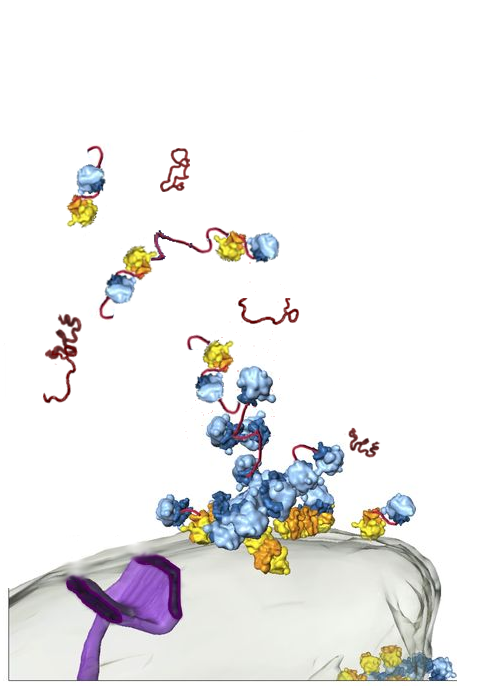
\includegraphics[width=0.4\textwidth]{Mitotransimport}
  \end{center}
  \caption{Selectively translated mRNA by heterogenous ribosomes}
  \label{selectivelytranslatedmrna}
\end{wrapfigure}

For it’s diverse role within the eukaryotic cell, its history is rooted in the kingdom prokaryota. It is considered to once have been an independent organism. Proof of the endosymbiotic theory of mitochondrial origin finally came into existence with the evidence of Mitochondria hosting it’s own DNA\textsuperscript{\cite{Gerst}}.
\vspace{3cm}



\clearpage

\paragraph{Some tips on how to use \LaTeX are here below:}
\newline
A cool experiment i tried is here (Sec:\ref{hefetrafo}), you should check it out.
\\
\vspace{2cm}

sometimes it helps to make \hspace{5mm} spaces...

\newline

The last page has a cool image I made using MS Paint: (Fig:\ref{selectivelytranslatedmrna}).

\paragraph{Accents and shit:}

Can you pronounce these?: \newline
{\"a} {\^e} {\`i} {\.I} {\o} {\'u} {\aa} {\c c} {\u g} {\l} {\~n} {\H o} {\v r} {\ss}
\\
\newline
Check out this \textit{\underline{\href{https://www.overleaf.com/learn/latex/List_of_Greek_letters_and_math_symbols#Greek_letters}{link}}} for how to write greek letters.
And this  \textit{\underline{\href{https://www.overleaf.com/learn/latex/Bold,_italics_and_underlining#Italicized_text}{link}}} about basic text formatting.\\

  \addcontentsline{toc}{chapter}

\chapter{Results}

I have no results for my thesis just yet, but hold on..
  \addcontentsline{toc}{chapter}

\chapter{Discussion}

Let's discuss my thesis...

How much do you like it?


  \addcontentsline{toc}{chapter}

\chapter{Materials and Methods}
I used may have used some materials, but i used a lot of methods
\newline
like..

\subsection{Transformation of \textit{S.cerevisiae} and selection}\label{hefetrafo}
After an intense workout.. the $\alpha$ Yeast found out that it could really get 6 bud abs.. This Yeast was the hottie of the a strain\\
  %\include{Chapter1}
  %\include{Chapter2}
\begin{appendix}


\chapter{Supplementary Figures}

Maybe I can show all the sequences here


\chapter{Genomes}

Should i be including the genomes of my organisms?


\end{appendix}



%\listoffigures
%  \markboth{List of figures}{List of figures}
%  \listoftables
%  \markboth{List of Tables}{List of Tables}
%  \cleardoublepage

  \backmatter
  \bibliographystyle{apa}
\bibliography{literatur}


  \markboth{}{}


  \addcontentsline{toc}{chapter}{\protect Acknowledgements}


\chapter*{Acknowledgments}

Danke Amit for the \LaTeX template

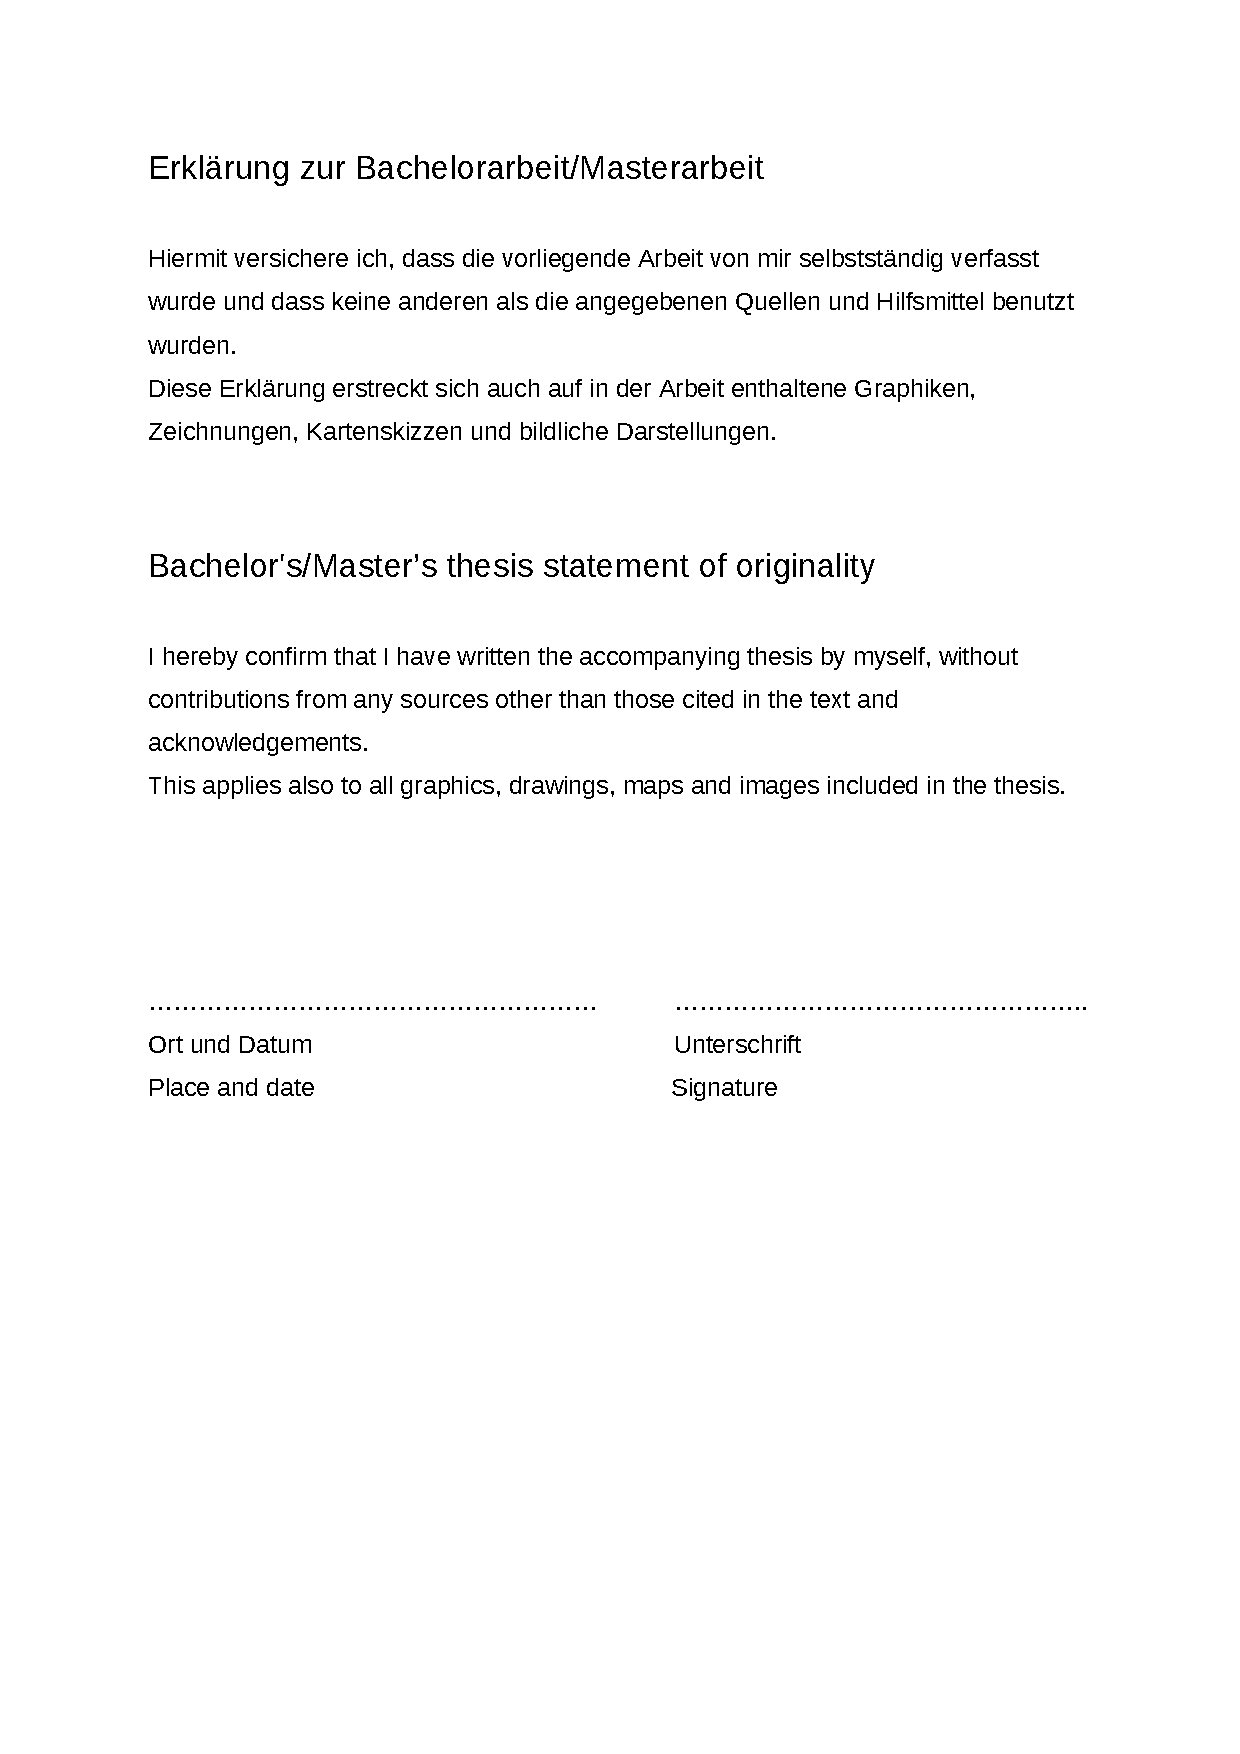
\includegraphics[width=\textwidth]{thesis_statement_original.pdf}
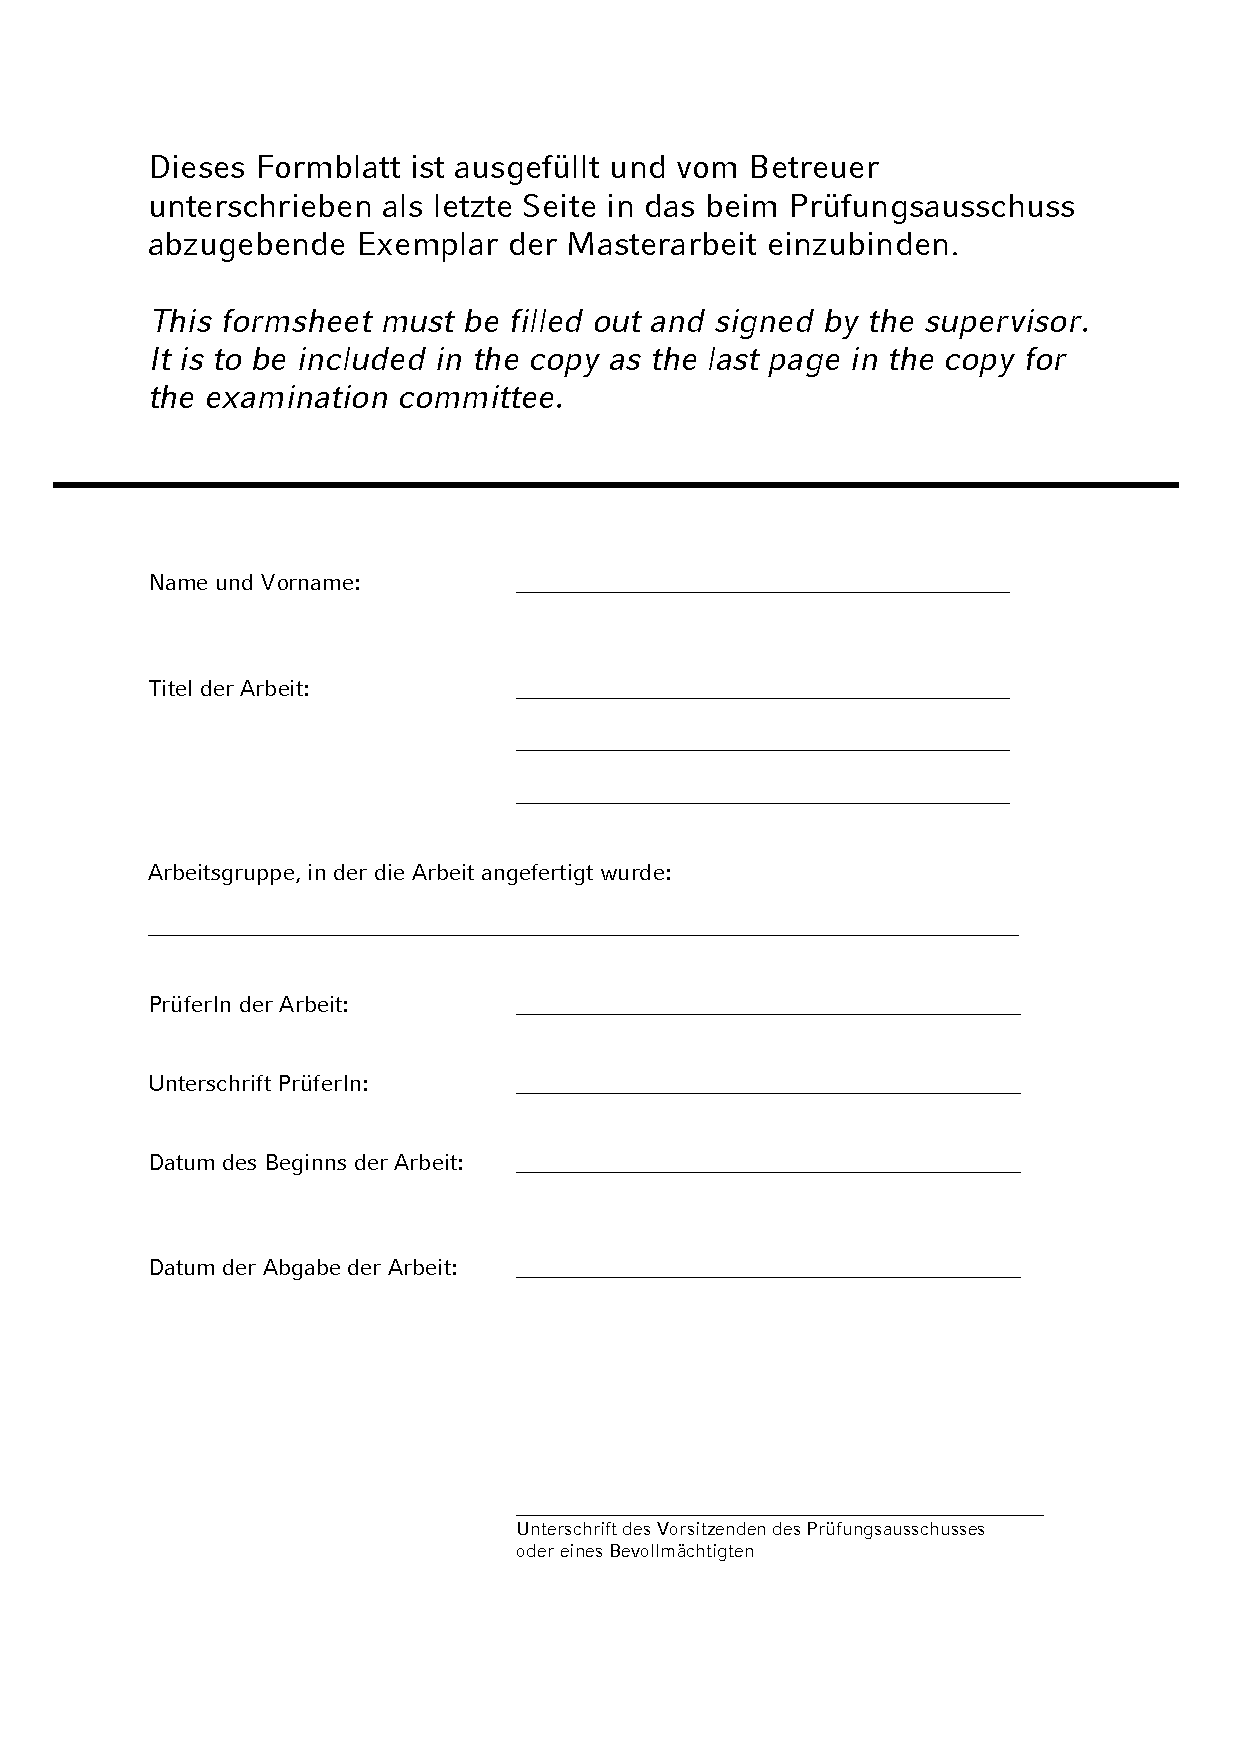
\includegraphics[width=\textwidth]{master-thesis-last-page.pdf}
 % \chapter*{Curriculum Vitae}

Amit Fenn

\vspace*{2.0cm}

\begin{tabular}{ll}

16.11.1989 & Cochin \\[1.5ex]
Schulzeit & Besuch der Schule in Ort \\[1.5ex]
 ... & ...
\end{tabular}

\end{document}
